\documentclass{article}
\usepackage{amsmath, amssymb}
\usepackage{tabularx}
\usepackage[english,polish]{babel}
\usepackage{polski}
\usepackage[top=3cm, bottom=2cm, left = 2cm, right = 2cm]{geometry}
\usepackage{graphicx} % Required for inserting images

\title{Obliczenia Naukowe Laboratorium Lista 5}
\author{Bartłomiej Puchała}
\date{December 2023}

\begin{document}

\maketitle

\section{Opis algorytmów}
\subsection{Algorytm eliminacji Gaussa}
Algorytm eliminacji Gaussa jest stosowany do rozwiązywania układu równań liniowych postaci: 
$$ Ax = b $$
dla danej macierzy współczynników $A \in \mathbb{R}^{n \times n}$ i wektora prawych stron $b \in \mathbb{R}^{n}$, $n \geq 4$. Zakładamy, że macierz $A$ jest nieosobliwa, tzn. jej wyznacznik $ \det(A) \neq 0$. Ten algorytm pozwala również na wyznaczenie rozkładu $LU$. Algorytm polega na doprowadzeniu macierzy $A$ do postaci trójkątnej(górnotrójkątnej), czyli na wyzerowaniu wszystkich komórek macierzy $A$ pod jej przekątną. W tym celu iteracyjnie będą wyznaczane ilorazy 
$$ I_{ik} = \frac{a_{ik}}{a_{kk}} $$ dla $ i = 1,2, \dots, n$ i $k = 1,2, \dots,n$, przez które wymnażane będą kolejne $k$-te równania. Tzn. chcąc wyzerować elementy w pierwszej kolumnie poniżej diagonali od wiersza $i$-tego odejmowany będzie wiersz $1$ pomonożony przez iloraz $I_{i1} = \frac{a_{i1}}{a_{11}}$. Przekształcenia dotyczyć będą również wektora prawych stron $b$, gdzie dla każdego i-tego wiersza zmieniać się będzie również wektor $b_i = b_i - I_{ik} * b_k$. A więc w celu wyzerowania elementów w pierwszej kolumnie poniżej diagonali dla każdego i-tego wiersza nowe wektory będą postaci $b_i = b_i - I_{i1} * b_1 $. Tak postępując otrzymany zostanie układ równań z macierzą trójkątną, który jest równoznaczny z układem pierwotnym. Można jednak zauważyć, że w przypadku wystąpienia jakiegokolwiek elementu $a_{kk}$ równego lub bliskiemu zeru na przekątnej algorytm może nie zadziałać lub zwrócić błędne wyniki. Aby temu zapobiec stosuje się 
\textbf{metodę częściowego wyboru}, która zapewnia numeryczną stabilność. Polega ona na wybraniu wiersza z największym elementem w danej kolumnie i zamianie miejscami z aktualnym wierszem, w którym znajduje się element główny(diagonalny). Dzięki temu zapewniona zostaje stabilność numeryczna algorytmu, lecz ma to skutek w postaci dłuższego czasu wykonywania. 
Do rozwiązania układu z macierzą trójkątną stosuje się \textbf{metodę podstawiania wstecz}, która polega na iteracyjnym wyznaczaniu kolejnych $x_i$, gdzie 
$$ x_i = \frac{b_i - \sum_{j=i+1}^{n} a_{j}*x_j }{a_{ii}} $$
W przypadku złożoności algorytmu eliminacji Gaussa, to doprowadzenie macierzy do postaci trójkątnej następuje w czasie $\mathcal{O}(n^3)$, natomiast rozwiązanie układu równań z taką macierzą zajmuje $\mathcal{O}(n^2)$, co daje sumaryczny koszt całego algorytmu w czasie $\mathcal{O}(n^3)$.

\subsection{Rozkład LU}
\textbf{Rozkład $LU$} polega na rozłożeniu macierzy kwadratowej $A$ na iloczyn dwóch maciery trójkątnych, dolnotrójkątnej $L$ o elementach na przekątnej równych 1 i wyzerowanych komórek macierzy nad przekątną, oraz macierzy górnotrójkątnej $U$ o wyzerowanych komórkach macierzy pod przekątną. Macierze te przedstawiają się następująco:
\vspace{15pt}
$$ L = \begin{pmatrix}
1 & 0 & \dots & 0 \\
I_{21} & 1 & \dots & 0 \\
\vdots & \vdots & \ddots & 0 \\
I_{n1} & I_{n2} & \dots & 1 \\
\end{pmatrix} $$

\vspace{15pt}
$$ U = \begin{pmatrix}
u_{11} & u_{12} & \dots & u_{1n} \\
0 & u_{22} & \dots & u_{2n} \\
\vdots & \vdots & \ddots & \vdots \\
0 & 0 & \dots & u_{nn} \\
\end{pmatrix} $$
\vspace{15pt}
Wtedy rozwiązanie równania 
$$ A * x = b $$
$$ L * U * x = b $$
sprowadza się do rozwiązania układu 2 układów trójkątnych:
\begin{enumerate}
    \item $ L * y = b $
    \item $ U * x = y $
\end{enumerate}
Rozwiązanie układu $ L * y = b$ odpowiada 
$$ y = L^{-1}b = L^{(n - 1)} \dots L^{(2)}L^{(1)}b = b^{(n)} $$
Macierz $U$ odpowiada macierzy oryginalnej $A$, tzn. komórki macierzy $U$ są uzyskiwane podczas algorytmu eliminacji Gaussa, a komórki macierzy $L$ są uzyskiwane z obliczonych mnożników użytych do zerowania elementów. Dla tego algorytmu istnieje również metoda z częściowym wyborem elementu głównego, która zapewnia numeryczną stabilność, tak jak w przypadku algorytmu eliminacji Gaussa. Złożoność algorytmu \textbf{rozkładu $LU$} jest równa złożoności algorytmu eliminacji Gaussa, wynosi $\mathcal{O}(n^3)$. Natomiast złożoność rozwiązania układu równań z macierzami $L, U$ jest równa $\mathcal{O}(n^2)$.

\subsection{Opis implementacji}
\subsubsection{Przechowywanie elementów}
W Julii istnieje w bibliotece standardowej pakiet SparseArrays, który umożliwia wydajne przechowywanie macierzy rzadkich, z wieloma zerowanymi elementami w postaci SparseMatrixCSC. Ta konstrukcja przechowuje 3 tablice o równych rozmiarach, pierwsza z nich informuje o numerach wierszy, druga o numerach kolumn, a trzecia z nich odpowiada wartościom na danym indeksie wiersza i kolumny w macierzy. Dzięki zastosowaniu tej konstrukcji można w sposób w miarę wydajny iterować po macierzy rzadkiej, nie pamiętając o komórkach zerowych.
\subsubsection{Optymalizacja pod treść zadania}
W problemie mamy do czynienia z macierzami rzadkimi i blokowymi, co pozwala na bardziej wydajną optymalizację powyższych algorytmów. \textbf{Warto zauważyć}, że skoro nasza macierz jest rzadka, to nie trzeba zerować całej kolumny pod przekątną w algorytmie eliminacji Gaussa, ponieważ większość komórek macierzy jest już wyzerowana. Dotyczy to również wierszy macierzy, tzn. w pierwszych wierszach zerowane elementy znajdują się na końcu wiersza, a wraz ze wzrostem numeru wiersza, te elementy zaczynają być zerowane na początku wiersza. \textbf{Optymalizacja w przypadku treści zadania} będzie polegała na \underline{ograniczeniu liczby wierszy}, dla których należy wyzerować komórki macierzy pod przekątną oraz \underline{ograniczeniu liczby kolumn} w procesie odejmowania wierszy.   
\subsection{Złożoność obliczeniowa}
\subsubsection{Analiza czasowa algorytmów bez wyboru elementu głównego}
\newpage
\begin{verbatim}
Dane wejściowe: A-macierz wejściowa, b-wektor prawych stron
    for i in 1:n-1
        for j in i+1:min(blockSize + i, n)
            factor = A![j, i] / A![i, i]
            A![j, i] = 0.0 # wyzerowanie kolumny pod przekątną

            for k in i+1:min(blockSize + i, n)
                A![j, k] -= factor * A![i, k]
            end
            b![j] -= factor * b![i]
        end
    end
\end{verbatim}
Algorytm zoptymalizowany eliminacji Gaussa ma złożoność $\mathcal{O}(nl^2)$, gdzie $n$ jest rozmiarem macierzy, a $l$ jest rozmiarem bloku. Algorytm można ograniczyć do złożoności $\mathcal{O}(n)$, jeżeli rozmiary macierzy blokowych($l$) są odpowiednio małe, tak że w porównaniu z $n$(rozmiarem macierzy) są na tyle małe, że pętlę wewnętrzną wyznaczającą ilorazy oraz pętlę wewnątrz niej iterującą  po kolumnach można ograniczyć do złożności $\mathcal{O}(1)$, czyli potraktować jako pewną ilość operacji stałych. Ten sam sposób został zastosowany do optymalizacji rozwiązywania równania Gaussa, który ma złożoność $\mathcal{O}(nl)$. W ten sposób cały algorytm rozwiązywania równania liniowego $A * x = b$ można ograniczyć do złożoności $\mathcal{O}(n)$. Podobna optymalizacja została wykorzystana dla rozkładu $LU$, poniżej:
\begin{verbatim}
function LU_decomposition!(
        L!::SparseMatrixCSC{Float64, Int64}, U!::SparseMatrixCSC{Float64, Int64},
        n::Int64, 
        blockSize::Int64
    ) 
    for i in 1:n-1
        L![i, i] = 1.0 # Diagonal as 1 in the L matrix
        for k in i+1:min(n, i + blockSize)
            factor = U![k, i] / U![i, i]
            L![k, i] = factor
            U![k, i] = 0.0
            for j in i+1:min(n, blockSize + i)
                U![k, j] -= factor * U![i, j]
            end
        end 
    end
    L![n,n] = 1.0
end
\end{verbatim}
Algorytm rozkładu $LU$ ma złożoność $\mathcal{O}(nl^2)$, ale skoro l jest stałą to cały algorytm ma złożoność czasową $\mathcal{O}(n)$.

\subsubsection{Analiza czasowa algorytmów z wyborem elementu głównego}
W przypadku algorytmów z wyborem elementu głównego złożoność czasowa będzie gorsza od algorytmów bez wyboru z powodu dodatkowych operacji, takich jak zamiana wierszy, dostosowanie wektora prawych stron, jak i również większy zakres pętli z powodu operacji zamiany wierszy.
\newpage
\begin{verbatim}
for i in 1:n-1
    row = 0.0
    col = 0.0

    for j in i:min(blockSize + i, n)
        if abs(A![pivots[j], i]) > col
            col = abs(A![pivots[j], i])
            row = j
        end
    end

    pivots[row], pivots[i] = pivots[i], pivots[row] # swap of rows

    for k in i+1:min(blockSize + i, n)
        factor = A![pivots[k], i] / A![pivots[i], i]
        A![pivots[k], i] = 0.0

        for m in i+1:min(2 * blockSize + i, n)
            A![pivots[k], m] -= factor * A![pivots[i], m]
        end

        b![pivots[k]] -= factor * b![pivots[i]]
    end
end
\end{verbatim}
Powyższy algorytm eliminacji Gaussa z wyborem elementu głównego będzie miał złożoność $\mathcal{O}(n * (l + l * 2l))$, czyli $\mathcal{O}(2nl^2)$, więc mimo że asymptotycznie złożoność jest taka sama jak w przypadku algorytmu bez wyboru elementu głównego i wynosi ona $\mathcal{O}(n)$, to stała tutaj jest większa, co wpłynie na gorszy czas wykonywania się algorytmu. Podobnie jest w przypadku rozkładu $LU$ z wyborem elementu głównego:
\begin{verbatim}
function LU_decomposition_with_partial_pivoting!(L!::SparseMatrixCSC{Float64, Int64}, U!::SparseMatrixCSC{Float64, Int64}, n::Int64, blockSize::Int64) 
    pivots = collect(1:n) # [1, 2, 3, ..., n] table of pivots
    for i in 1:n-1
        row = 0.0
        col = 0.0
        L![i, i] = 1.0

        for j in i:min(blockSize + i, n)
            if abs(U![pivots[j], i]) > col
                col = abs(U![pivots[j], i])
                row = j
            end
        end
        pivots[row], pivots[i] = pivots[i], pivots[row] # swap of rows
        for k in i+1:min(n, i + blockSize)
            factor = U![pivots[k], i] / U![pivots[i], i]

            L![pivots[k], i] = factor
            U![pivots[k], i] = 0.0

            for j in i+1:min(n, 2 * blockSize + i) # 2* because of swapped rows
                U![pivots[k], j] -= factor * U![pivots[i], j]
            end
        end 
    end
    L![n, n] = 1.0
    return pivots
end
\end{verbatim}
Powyższy algorytm ma również złożoność czasową $\mathcal{O}(2nl^2)$, czyli jeżeli $l$ jest stałą to  $\mathcal{O}(n)$.
\subsection{Złożoność pamięciowa}
\vspace{10pt}
\subsubsection{Złożoność pamięciowa algorytmów bez wyboru elementu głównego}
\begin{enumerate}
    \item Każda z $v$ macierzy $A_{k}$ potrzebuje $l^2$ liczb do zapisu
    \item Każda z $v - 1$ macierzy $B_{k}$ potrzebuje $l$ liczb do zapisu 
    \item Każda z $v-1$ macierzy $C_{k}$ potrzebuje $\frac{l(l+1)}{2}$ liczb do zapisu
\end{enumerate}
Złożoność pamięciowa w sumie wynosi $\mathcal{O}(ln)$, a l jest stałą, więc wynosi $\mathcal{O}(n)$.
\subsubsection{Złożoność pamięciowa algorytmów z wyborem elementu głównego}
\begin{enumerate}
    \item Każda z $v$ macierzy $A_{k}$ potrzebuje $l^2$ liczb do zapisu
    \item Każda z $v - 1$ macierzy $B_{k}$ potrzebuje $l$ liczb do zapisu 
    \item Każda z $v-1$ macierzy $C_{k}$ potrzebuje $l^2$ liczb do zapisu
    \item Permutacja $p$(pivots) potrzebuje $n$ liczb do zapisu
\end{enumerate}
Złożoność pamięciowa w sumie wynosi $\mathcal{O}(ln)$, a l jest stałą, więc wynosi $\mathcal{O}(n)$.
\subsection{Algorytmy rozwiązywania po eliminacji Gaussa oraz rozkładzie LU}
\vspace{10pt}
\subsubsection{Algorytmy rozwiązujące eliminację Gaussa}
\begin{verbatim}
function solve_gauss(A::SparseMatrixCSC{Float64, Int64},
    b::SparseVector{Float64, Int64},
    blockSize::Int64, n::Int64)
    
    x = zeros(Float64, n)
    x[n] = b[n] / A[n, n]

    for i in n-1:-1:1
        current_sum = 0
        for j in i+1:min(n, i + blockSize)
            current_sum += x[j] * A[i, j]
        end
        x[i] = (b[i] - current_sum) / A[i, i]
    end
    return x
end
\end{verbatim}
\newpage
\begin{verbatim}
function solve_gauss_with_partial_pivoting(A::SparseMatrixCSC{Float64, Int64}, 
b::SparseVector{Float64, Int64}, blockSize::Int64, n::Int64, pivots::Vector{Int64})
    x = zeros(Float64, n)
    for k in 1:n-1 # dostosowanie wektora prawych stron b w trakcie eliminacji wstecznej
        for i in k+1:min(n, k + 2 * blockSize)
            b[pivots[i]] -= A[pivots[i], k] * b[pivots[k]]
        end
    end

    for i in n:-1:1
        currentSum = 0
        for j in i+1:min(n, i + 2 * blockSize)
            currentSum += A[pivots[i], j] * x[j]
        end
        x[i] = (b[pivots[i]] - currentSum) / A[pivots[i], i]
    end
    return x
end
\end{verbatim}
\vspace{5pt}
\subsubsection{Algorytmy rozwiązujące rozkład $LU$}
\begin{verbatim}
function solveLU(L::SparseMatrixCSC{Float64, Int64}, U::SparseMatrixCSC{Float64, Int64},
b::SparseVector{Float64, Int64}, n::Int64, blockSize::Int64)
    x = zeros(Float64, n)

    for i in 1:n-1 # Rozwiązanie równania Ly = b
        for j in i+1:min(n, blockSize + i)
            b[j] -= L[j, i] * b[i]
        end
    end

    for i in n:-1:1 # Rozwiazanie rownania Ux = y
        currentSum = 0
        for j in i+1:min(n, i + blockSize)
            currentSum += U[i, j] * x[j]
        end
        x[i] = (b[i] - currentSum) / U[i, i]
    end
    return x
end
\end{verbatim}
\newpage
\begin{verbatim}
function solveLU_with_partial_pivoting(L::SparseMatrixCSC{Float64, Int64}, 
U::SparseMatrixCSC{Float64, Int64},
b::SparseVector{Float64, Int64}, n::Int64, blockSize::Int64, pivots::Vector{Int64})
    x = zeros(Float64, n)
    y = zeros(Float64, n)

    for i in 1:n # Rozwiązanie równania Ly = b
        y[pivots[i]] = b[pivots[i]]
        for j in 1:i-1
            y[pivots[i]] -= L[pivots[i], j] * y[pivots[j]]
        end
    end

    for i in n:-1:1 # Rozwiazanie rownania Ux = y
        currentSum = 0
        for j in i+1:min(n, i + 2 * blockSize)
            currentSum += U[pivots[i], j] * x[j]
        end
        x[i] = (y[pivots[i]] - currentSum) / U[pivots[i], i]
    end
    return x
end
\end{verbatim}
\section{Wyniki}
\subsection{Metoda testowania}
Testy polegały na sprawdzeniu zależności od czasu oraz od pamięci poszczególnych algorytmów. Polegały one na przeprowadzeniu 10 iteracji, w każdej z nich generowana była macierz rzadka funkcją \textbf{blockmat}, następnie dla każdego algorytmu wyliczany był wektor prawych stron $b$ i dla tak zadanych danych oraz stałego rozmiaru bloku i zwiększających się rozmiarów macierzy zostały przeprowadzone następujące testy, z których otrzymano następujące wykresy.

\begin{figure}[htpb] 
    \centering
    \includegraphics[width=0.7\textwidth, height=7.5cm]{"gauss_plot.png"}
    \caption{Czas wykonania gauss}
    \label{eeexd}
\end{figure}

\begin{figure}[htpb]
    \centering
    \includegraphics[width=0.7\textwidth, height=8cm]{"lu_plot.png"}
    \caption{Czas wykonania rozkładu LU}
    \label{lu_label}
\end{figure}

\begin{figure}[htpb] 
    \centering
    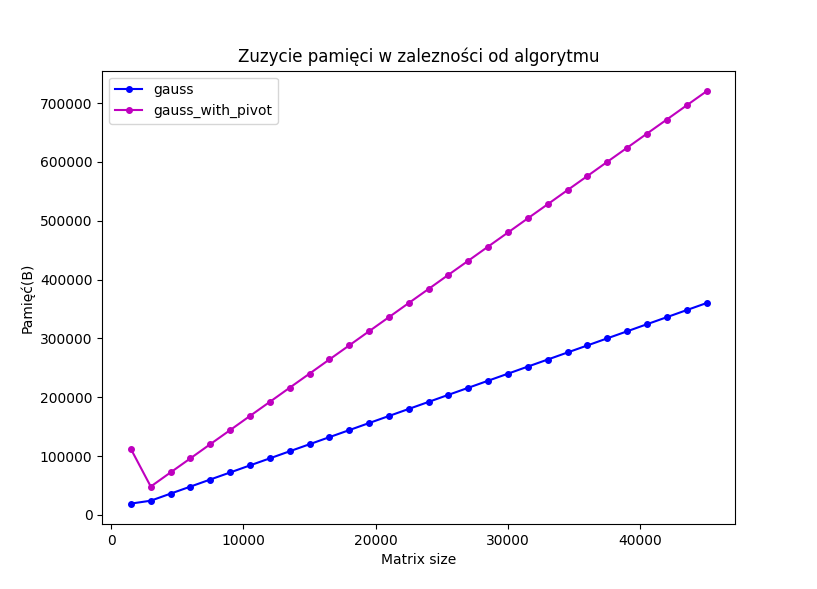
\includegraphics[width=0.7\textwidth, height=8cm]{gauss_memory.png}
    \caption{Zużycie pamięci gauss}
    \label{xxx}
\end{figure}

\begin{figure}[htpb] 
    \centering
    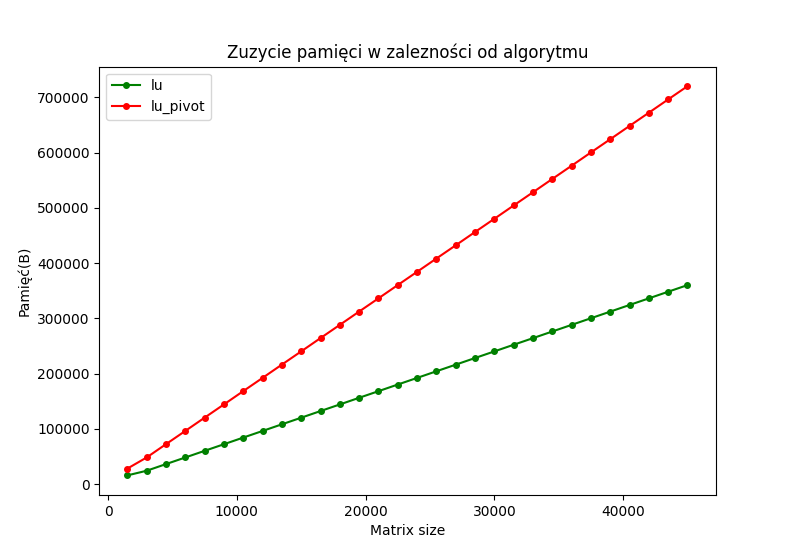
\includegraphics[width=0.7\textwidth, height=8cm]{lu_memory.png}
    \caption{Zużycie pamięci rozkładu LU}
    \label{lu_memory}
\end{figure}

\begin{figure}[htpb] 
    \centering
    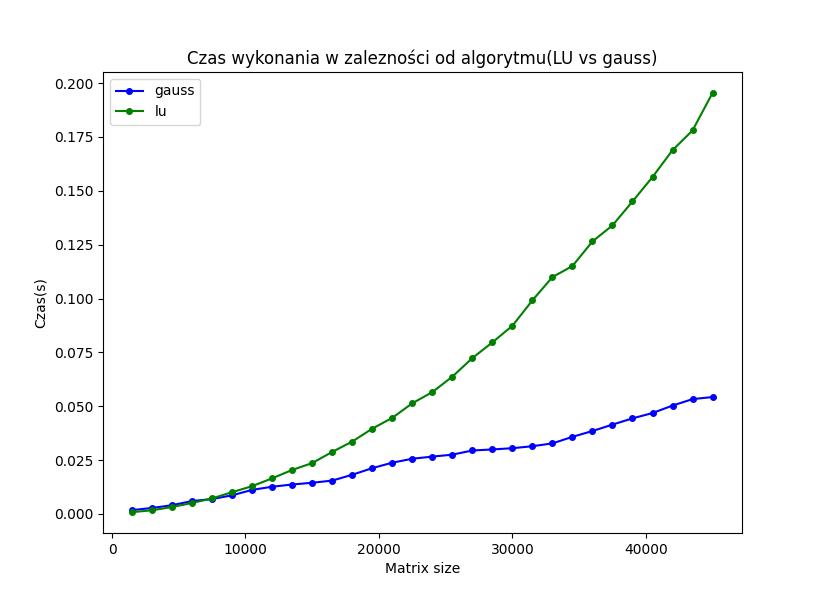
\includegraphics[width=0.7\textwidth, height=8cm]{gauss_lu.png}
    \caption{Czas wykonania(gauss vs LU)}
    \label{gauss_vs_lu}
\end{figure}

\section{Wnioski}
Odpowiednio dostosowana implementacja dla zadanego typu zadania pozwala na optymalizację czasu oraz pamięci wykonywania danego problemu, co pozwala na efektywne rozwiązywanie zadanych problemów.
\end{document}
